\chapter[The Physics of The \Zprime~Boson]{The Physics of the \Zprime~Boson}
\label{chap:Zp}

\noindent In the search for physics BSM at the LHC one of the most exciting possibilities 
is the observation of neutral vector bosons with masses in the range of 
the \TeV's, generally known as \Zprime. Many models of physics 
BSM include this kind of states as a result of the breaking of higher symmetries upon 
which the models are built. \\

\noindent The Standard Model is a gauge field theory that has as its underlying symmetry 
group $G_{SM} = SU(3)_{C}\otimes SU(2)_{L} \otimes SU(1)_{Y}$ and a breaking mechanism 
mediated by the Higgs field, that leaves, as the remaining symmetry the group,
$SU(3)_{C}\otimes SU(1)_{EM}$. This is an example of how the breaking of a larger symmetry 
results on one or more $U(1)$ factors. These $U(1)$ factors are associated to gauge
bosons that can be massive.\\

\noindent Models beyond the SM have larger symmetry groups than $G_{SM}$, and various symmetry breaking 
mechanisms that include $G_{SM}$ as remaining symmetry. But, in many of these 
scenarios extra $U(1)$ factors can also remain. They would be associated 
to neutral and massive vector bosons. For instance, a group $SU(N)$ can 
be broken by a Higgs-like mechanism, and the unbroken subgroup could contain up to
N-1 $U(1)$ factors \cite{Langacker:2008yv}. Therefore, the emergence of remaining 
$U(1)$ symmetries in the breaking of larger groups is a common feature 
of models BSM. This is why experimental signatures of new physics 
would, most likely, involve neutral vector bosons.\\
% 
\noindent In the case of grand unified theories (GUT) groups like $SU(5)$, $SO(10)$ or $E_{6}$ have been
used as the main symmetry whose breaking would, eventually, take us to $G_{SM}$. But, this
does not discard the presence of extra $U(1)$ factors, whose associated 
gauge bosons have large enough masses, so that they have not 
been observed so far, but that could be within the reach of the LHC 
experiments. \\

\noindent Not just plain GUT theories, but also superstring theories have large symmetry groups 
that break into $G_{SM} \otimes U(1)^{n}$ with $n \geq 1$. A similar situation can be found in 
GUT-SUSY models. Even some versions of theories with extra space dimensions involve
massive \Zprime~in their particle spectra. \\

\noindent The breaking of the larger symmetry, resulting in $U(1)$ factors, would typically demand 
for an extended Higgs sector, that would have implications in particle physics
and cosmology. This is why the observation of a \Zprime~would provide very valuable
information about the new physics involved.\\

\noindent The theoretical implications of the discovery of a \Zprime~at the LHC could range 
from flavor changing neutral current processes, rare B decays, production of other 
massive exotic particles in the decay chain, neutrino masses, etc.\\

\section{\Zprime~Couplings}
\label{sec:ZprimeCoupling}

\noindent To understand how a new \Zprime~field would couple to other fields, specially
to those of the SM, one can look at the case of the two known  neutral vector 
bosons: $A_{\mu}$ and $Z_{1\mu}$ (here a sub-index 1 has been included 
to distinguish it from new Z-like states). The interaction of these 
fields with fermions is given by \cite{Langacker:2008yv}:

\begin{equation}
 g J_{3}^{\mu} W_{3\mu} + g\prime J_{\nu}^{\mu} B_{\mu} = e J_{em}^{\mu} A_{\mu} + g_{1} J_{1}^{\mu} Z_{1\mu} \; ,
\end{equation}

\noindent where $g$ and $g\prime$ are the gauge couplings associated
to $SU(2)$ and $U(1)_{Y}$ respectively. \\

\noindent Here we have the interaction written in two basis:
\begin{itemize}
 \item the gauge-eigenstates basis: $W_{3\mu}$, $B_{\mu}$,
 \item the mass-eigenstates basis: $A_{\mu}$, $Z_{1\mu}$,
\end{itemize}
\noindent related by:

\begin{equation}
\begin{split}
 A_{\mu} &= \sin \theta_{W} W_{3\mu} + \cos \theta_{W} B_{\mu} \; , \\
 Z_{1\mu} &= \cos \theta_{W} W_{3\mu} - \sin \theta_{W} B_{\mu} \; ,
\end{split}
\end{equation}

\noindent where,

 \begin{equation}
 \begin{split}
  \tan \theta_{W} = \frac{g\prime}{g} \; ; \;  e = g \sin \theta_{W} \; , \\
    g_{1}^{2} = g^{2} + g\prime^{2} = \frac{g^{2}}{\cos ^{2} \theta_{W}} \; .
 \end{split}
 \end{equation}

\noindent The fermion currents are given by:

\begin{equation}
\begin{split}
 J_{3}^{\mu} &= \sum_{i} \bar{f}_{i} \gamma^{\mu} \left[t_{3iL} P_{L} + t_{3iR} P_{R} \right] f_{i} \; , \\
 J_{Y}^{\mu} &= \sum_{i} \bar{f}_{i} \gamma^{\mu} \left[y_{iL} P_{L} + y_{iR} P_{R} \right] f_{i} \; ,
\end{split}
\end{equation}

\noindent in the gauge-eigenstates basis, and by:

\begin{equation}
\begin{split}
 J_{em}^{\mu} &= \sum_{i} q_{i} \bar{f}_{i} \gamma^{\mu} f_{i}  \; , \\
 J_{1}^{\mu} &= \sum_{i} \bar{f}_{i} \gamma^{\mu} \left[\epsilon_{L}^{1}(i) P_{L} + \epsilon_{R}^{1}(i) P_{R} \right] f_{i} \; , 
\end{split}
\end{equation}

\noindent in the mass-eigenstates basis.\\

\noindent Here $f_{i}$ are the fermion fields, $P_{L,R}= (1 \pm \gamma^{5})/2$ and $t_{3iL,R}$ is the third component
of weak isospin of the fermion field, given by:

 \begin{equation}
 \begin{split}
 t_{3u L} &= t_{3\nu L} = +\frac{1}{2}  \; ,  \\
 t_{3d L} &= t_{3 e L} = -\frac{1}{2}   \; ,   \\
 t_{3iR} &= 0 \\  \; .
 \end{split}
 \end{equation}

 \noindent The $y_{iL,R}$ are the weak hypercharges given by:
 
 \begin{equation}
  t_{3iL} + y_{iL} = t_{3iR} + y_{iR} = q_{i} \; ,
 \end{equation}

 \noindent where $q_{i}$ is the electric charge of the fermion field.\\
 
 \noindent The chiral couplings $\epsilon_{L}^{1}(i)$ and $\epsilon_{R}^{1}(i)$ are given by:
 
 \begin{equation}
 \begin{split}
 \epsilon_{L}^{1}(i) &= t_{3i L} -\sin^{2} \theta_{W} q_{i} \; ,  \\
 \epsilon_{R}^{1}(i) &= t_{3i R} -\sin^{2} \theta_{W} q_{i} \; . 
 \end{split}
 \end{equation}
 
 \noindent In the case of extra $U(1)^{\prime}$ symmetries, the interaction 
 terms become:
 \begin{equation}
  e J_{em}^{\mu} A_{\mu} + \sum_{\alpha = 1}^{n+1} g_{\alpha} J^{\mu}_{\alpha}Z_{\alpha \mu} \; ,
  \label{eq:couplings}
 \end{equation}

 \noindent where $n$ is the number of extra $U(1)^{\prime}$ factors; 
 $g_{1}$, $Z_{1\mu}$, and $J_{1\mu}$ are the gauge coupling, the boson field, and 
 the SM neutral current, respectively. Similarly, $g_{\alpha}$, $Z_{\alpha \mu}$,
 $\alpha = 2 \cdots n+1 $, are the gauge couplings and boson fields
 for the additional $U(1)^{\prime}$ factors. The currents in equation
 \ref{eq:couplings} are:

 \begin{equation}
 \begin{split}
J_{\alpha}^{\mu}   &= \sum_{i} \bar{f}_{i} \gamma^{\mu} \left[\epsilon_{L}^{\alpha} P_{L} + \epsilon_{R}^{\alpha} P_{R} \right] f_{i} \; ,  \\
                   &= \sum_{i} \bar{f}_{i} \gamma^{\mu} \left[g_{V}^{\alpha}(i) - g_{A}^{\alpha}(i)\gamma^{5} \right] f_{i} \; ,
 \end{split}
 \end{equation}

 \noindent where, the chiral couplings $\epsilon_{L,R}^{\alpha}(i)$ are 
 respectively the $U(1)_{\alpha}$ charges of the left and right 
 handed components of fermion $f_{i}$, and $g_{V,A}^{\alpha}(i) = \epsilon_{L}^{\alpha}(i) \pm \epsilon_{R}^{\alpha}(i)$
  are the corresponding vector and axial couplings. \\

\noindent Following a spontaneous breaking mechanism similar to the one of 
the SM, complex $SU(2)$ scalar multiplets $\phi_{i}$ are included:

\begin{equation}
 \phi_{i} = 
\left(
 \begin{matrix}
  \phi^{+}_{i} \\
  \phi^{0}_{i} \\
 \end{matrix}
\right) \; .
 \end{equation}

 \noindent If the neutral component of $\phi_{i}$ acquires a vacuum expectation 
 values (VEV), different from zero, $A_{\mu}$ would remain massless,
 while the $Z_{\alpha \mu}$ develop mass terms of the form:
 
 \begin{equation*}
  \frac{1}{2}M_{\alpha \beta}^{2} Z_{\alpha \mu} Z_{\beta}^{\mu} \; ,
 \end{equation*}

 \noindent where $M_{\alpha \beta}$ is the mass matrix for the $Z$ vector
 bosons. \\
 
 \noindent In the case $n = 1$ (only one \Zprime), the matrix takes the form:
 
\begin{equation}
 M_{\alpha \beta} = 
\left(
 \begin{matrix}
  M_{Z 0}^{2}  & \Delta^{2}     \\
  \Delta^{2}   & M_{Z\prime}^{2} \\
 \end{matrix}
\right) \; , 
 \end{equation}
 
\noindent This matrix can be diagonalized with the rotation:
 \begin{equation}
 U = 
\left(
 \begin{matrix}
   \cos \theta  & \sin \theta \\
   -\sin \theta & \cos \theta \\
 \end{matrix}
\right) 
 \end{equation}
\begin{equation}
 \theta = \frac{1}{2} \arctan \left( \frac{2 \Delta^{2}}{M_{Z 0}^{2} - M_{Z\prime}^{2}} \right) \; .
\end{equation}
\noindent The mass eigenvalues are given by:
\begin{equation}
 M_{1,2}^{2} = \frac{1}{2} \left[ M_{Z 0}^{2} + M_{Z\prime}^{2} \mp \sqrt{(M_{Z\prime}^{2} - M_{Z 0}^{2})^{2}+4 \Delta^{4}} \right]  \; ,
\end{equation}

\noindent where $\Delta^{2}$ is a quantity that depends on the model, and on the VEV of the 
Higgs doublets. If $M_{Z\prime} >> M_{Z 0}$, $|\Delta| \;$ then

\begin{equation}
\begin{split}
 M_{1}^{2} \sim M_{Z 0}^{2} - \frac{\Delta^{4}}{M_{Z\prime}^{2}} \sim M_{Z 0}^{2} << M_{2}^{2} \; , \\
 M_{2}^{2} \sim M_{Z\prime}^{2} \; .
\end{split}
\end{equation}

\noindent In summary, due to the needed symmetry breaking, there is a mass mixing between
$Z^{0}$ and \Zprime. But if $M_{Z\prime} >> M_{Z 0}$, the mixing is small \cite{ZprimeMixing}.\\

\noindent Another source of mixing comes from the kinetic terms. The most general form of these terms is:

\begin{equation}
-\frac{1}{4}F_{\alpha}^{\nu\mu}F_{\alpha\nu\mu} -\frac{1}{4}F_{\beta}^{\nu\mu}F_{\beta\nu\mu} -\frac{c_{\alpha\beta}}{2}F_{\alpha}^{\nu\mu}F_{\beta\nu\mu} \; , \\
\end{equation}

\noindent where $F_{\alpha\nu\mu} = \partial_{\mu}Z_{\alpha \nu} - \partial_{\nu}Z_{\alpha \mu}$. As one can see, there is a 
cross term that generates a kinetic mixing between the fields. In the case 
of $n = 1$,  one can write $c_{\alpha\beta} = \sin \chi$, and kinetic
mixing generates a transformation:

\begin{equation}
 \left(
 \begin{matrix}
  Z_{1 \mu}  \\
  Z_{2 \mu} \; ,
 \end{matrix}
\right)
 = 
\left(
 \begin{matrix}
  1    & -\tan \chi      \\
  0    & \frac{1}{\cos \chi} \\
 \end{matrix}
\right)
 \left(
 \begin{matrix}
  \hat{Z}_{1 \mu}  \\
  \hat{Z}_{2 \mu} \\
 \end{matrix}
\right) \; ,
 \end{equation}

 \noindent that, in turn, will affect the mass eigenvalues. Again, in most of the 
 cases, $\chi$ is small, and the effect over the mass 
 eigenvalues is also small.

\section{A Heavy Gauge Boson \Zprime~in BSM Theories}
\label{sec:Models}

As mentioned, there are many theoretical models 
that include \Uprime~symmetries. These models differ in coupling 
constants, even though most of them assume the electroweak
strength values of the SM. The other aspect that 
differentiates between models is the symmetry 
breaking scheme and scale. Some examples of these kinds 
of theories are:

\begin{itemize}
 \item \textit{The Sequential Standard model (SSM)}: is a simplified model in which the \Zprime~has the same 
couplings and quantum numbers as the $Z^{0}$, but higher mass. It serves as a 
reference for experimental searches \cite{bib:SSM}.

 \item \textit{$E_{6}$ models}: These models are based on the $E_{6}$ group as gauge symmetry,
which breaks at GUT scale down into the SM gauge group and extra $U(1)$ symmetry 
groups, usually two of them. Depending on the features of the 
particular model, one can have $M_{Z\prime} \sim$ \TeV~\cite{E6models}.

 \item \textit{Left-Right symmetric models}: These models involve the gauge group $SU(2)_{L}\times SU(2)_{R} \times U(1)_{B\cdot L}$,
where $B$ and $L$ refer to Baryon and Lepton numbers. These kind of theories 
predict a new heavy \Zprime, but also new heavy $W^{\pm \prime}$ bosons \cite{leftrightmodels}. The new 
$W^{\prime}$ is always lighter than the \Zprime, providing a good experimental test.

 \item \textit{Technicolor models}: This kind of models include a new gauge force with properties 
similar to those of QCD. They predict new particles, such as technigluons and 
techniquarks. In extended versions, new gauge bosons couple to the 
SM fermions and the technifermions. A \Zprime~boson emerges from the symmetry 
breaking induced by technifermion condensates. This boson couples only to 
left handed fermions, and has enhanced couplings to fermions of the 
third generation. Therefore, the search for \Zprimetotautau~is
of particular importance for testing these models \cite{Technicolor}.

 \item \textit{Topcolor assisted technicolor models}: TAT models interpret the large 
value of the top quark mass as an evidence 
of a dynamical electroweak breaking mechanism that depends on the fermion 
generation. They assume an extended gauge sector of the form 
$SU(3)_{1}\times SU(3)_{2} \times U(1)_{1}\times U(2)_{2}$. Fermions of
the first and second generation transform under $U(1)_{1}$, while 
fermions of the third generation transform under $U(2)_{2}$. The \Zprime~arises 
from the $U(1)_{1}$ group. In these models the couplings to fermions
of the third generation are also enhanced \cite{ZprimeThirdGeneration,TAT}.

 \item \textit{Little Higgs models}: These are the most popular non-GUT models that include 
new heavy gauge bosons. New $W^{\prime}$ and \Zprime~bosons, with masses of 
the order of \TeV~are predicted as a result of the symmetry 
breaking of a $[SU(2)_{L}\times U(1)]^{2}$ gauge group that is part of the models \cite{LittleHiggs1,LittleHiggs2}.

\end{itemize}







% \subsection{Sequential Standard Model}
% \label{subsec:SSM}
% 
% \subsection{Non Universal \Zprime~Model}
% \label{subsec:TAT}

 
% 
% 
% \section{Theoretical Motivation}
% \label{sec:Motivation}


\section{Searches for \Zprime~Gauge Bosons}
\label{sec:Searches}

% Several BSM theories predict the existence of \Zprime~bosons as a
% manifestations of an extended symmetry groups, as was described above.
% Since this heavy neutral bosons

The \Zprime~bosons predicted by the many theoretical models mentioned above
 would have couplings to SM quarks, therefore they might be 
produced by hadron colliders and might be observed directly  as 
additional resonances in invariant mass distribution plots. Tevatron and LHC 
experiments have performed direct searches for \Zprime~resonances. LEP 
performed indirect searches, since the \Zprime~could not be produced on-shell, given the 
energy range reached by this accelerator (209 \GeV). The searches 
performed by the LEP, Tevatron, and LHC experiments have not shown any
evidence of a \Zprime~boson, and have constrained its existence on a wide
range of mass. In this section the state of the art in the indirect and direct
experimental searches for the \Zprime~boson are presented.

%indirect (section \label{subsec:IndirectSearches}) direct (section \label{subsec:DirectSearches}). 

\subsection{Indirect Searches}
\label{subsec:IndirectSearches}

LEP experiments performed indirect searches using accurate electroweak 
measurements around the Z peak, looking for interference effects that might reveal a 
possible mixed state between \Zprime~and Z bosons, predicted by some BSM scenarios. LEP experiments 
looked for evidences of the mixing, using measurements of cross sections
and forward-backward asymmetries in the di-lepton channels. The LEP experiments did not report
any deviation from the SM expectations, and indirect limits on the \Zprime~mass were 
established (see Table \ref{LEPZprime}). The results were obtained with  the data sample 
collected by the four LEP experiments, using $e^{+}e^{-}$ collisions data \centermassenergy~of $209$ \GeV~\cite{LEP1,LEP2}.

 \begin{table}[ht]
\begin{center}
\begin{tabular}{|c|c|c|c|c|}
  \hline
  % after \\: \hline or \cline{col1-col2} \cline{col3-col4} ...
  Z$'$ model                        &  $\chi$ & $\psi$ & $\eta$ & SSM  \\ \hline\hline
  Mass limit for Z$'$ (\GeV)         &   673   &   481  &   434  & 1787 \\
  \hline
\end{tabular}
\end{center}
\caption{The 95$\%$ confidence level lower limits on the Z$'$ mass for $\chi$, $\psi$, $\eta$ and SSM models
set by the experiments ALEPH, DELPHI, L3 and OPAL \cite{LEP2}.}\label{LEPZprime}
\end{table}

\subsection{Direct Searches}
\label{subsec:DirectSearches}

Direct searches for a \Zprime~boson have been performed by the CDF \cite{CDFZprimedielectronbib,CDFZprimedimuonbib,CDFZprimeditaubib,CDFZprimeditopbib}
and D0 \cite{D0Zprimesearchesbib,D0Zprimetodielectronbib,D0Zprimeditopbib} experiments at the Tevatron, and 
by the CMS \cite{CMSZprimetodileptonrun1run2, CMSZprimetodileptonrun1, CMSZprimetodileptonrun1sqrt7, CMSZprimetotautaurun1, CMSZprimetotautauemu, 
CMSZprimetotautau2015, CMSZprimeto4leptons, CMSZprimeHplusZ, CMSZprimetotoptoprun1, CMSZprimetodibjetsrun1, CMSZprimedijetrun2} and
ATLAS \cite{ATLASZprimetodileptonrun2, ATLASZprimetodilepton2015, ATLASZprimetodilepton2012, ATLASZprimetodileptonrun1, ATLASZprimetotautau2016,
ATLASZprimetotautau2015, ATLASZprimetotautaurun1, ATLASZprimetotautau2011, ATLASZprimetojet2015, ATLASZprimetobjet2015} experiments at
the LHC. The \Zprime~have been searched in many channels, since there are several theoretical models and several couplings in 
each scenario. The Sequential Standard Model, or SSM, is one of the most frequently used models since it predicts 
a \ZprimeSSM~whose couplings are identical to those of the Z boson (see Section \ref{sec:Models}). Furthermore,  other searches
have included hypothetical \Zprime~bosons coming from in GUT theories, such as the \Zprimepsi~and \Zprimechi~bosons which arise 
from a symmetry breaking of the E$_{6}$ group, and the \Zprimeeta~boson which comes from a breaking symmetry of 
the SO(10) group in GUT scales (see Section \ref{sec:Models}). Additionally, models where the \Zprime~boson decays 
preferentially to the third generation of leptons (see Section \ref{sec:Models}), as the topcolor-assisted 
technicolor (TAT) models, have motivated the searches in the di-tau channel.\\

\noindent A direct evidence of a \Zprime~boson should show up as a heavy resonance in 
the mass spectrum of its decay products, since it would decay into two leptons or jets
with high momentum and opposite charge. No direct evidence has 
been found yet and its existence has been excluded on a wide range of mass. The constraints 
on the \Zprime~mass are usually presented as limits in the production cross section
times the branching fraction of its decay products, for instance: $\sigma ( pp \rightarrow Z^{\prime})\times B(Z^{\prime} \rightarrow \mu\mu)$. Several 
direct searches have been performed according to its decay products:

\begin{itemize}
 \item \textbf{Di-lepton searches (\Zprimetoll~channel, $\ell=e, \mu$).}\\

\noindent The \Zprimetoll~channel has been widely explored since light leptons
are usually reconstructed with high efficiencies in a large range of acceptance, which leads
to a high resolution in the di-lepton invariant mass; additionally, the di-lepton channel
has a negligible QCD background contamination. These features makes this channel the most 
sensitive one, providing the tightest exclusion limits on the \Zprime~mass. The main background comes 
from Drell-Yan (DY) processes since they have the same topology than the 
hypothetical \Zprime~events, and their reconstructed mass distribution can extend to large values where the
\Zprime~boson is expected; therefore, DY processes are an irreducible source of background. However, since 
this background have been very well studied and understood, its contribution is well modeled and simulated. \\

\noindent The CDF and D0 experiments performed the searches in the di-lepton
channel \cite{CDFZprimedielectronbib,CDFZprimedimuonbib,D0Zprimetodielectronbib},
using data samples of $p\bar{p}$ collisions at $\sqrt{s}=$ 1.96 \TeV. In the di-electron 
channel, CDF used a sample with an integrated luminosity of 1.3 fb$^{-1}$ and did not report a 
significant excess for the masses below 923 \GeV~ in the case of the \ZprimeSSM~and for masses below 822 \GeV~ 
in the case of the \Zprimepsi~(see Figure \ref{CDFD0dielectronresult}, left). The data collected by D0, with 
an integrated luminosity of 5.4 fb$^{-1}$, excluded the existence of the \ZprimeSSM~for masses below 1023 \GeV~
and the \Zprimepsi~for masses below 891 \GeV~ (see Figure \ref{CDFD0dielectronresult}, right). The CDF Collaboration 
also searched in the \Zprimetomumu~channel with an integrated luminosity of 4.6 fb$^{-1}$, which 
resulted in a lower limit of 1071 \GeV~ for the \ZprimeSSM~mass \cite{CDFZprimedimuonbib}. \\

\begin{figure}[ht]
    \begin{center}
      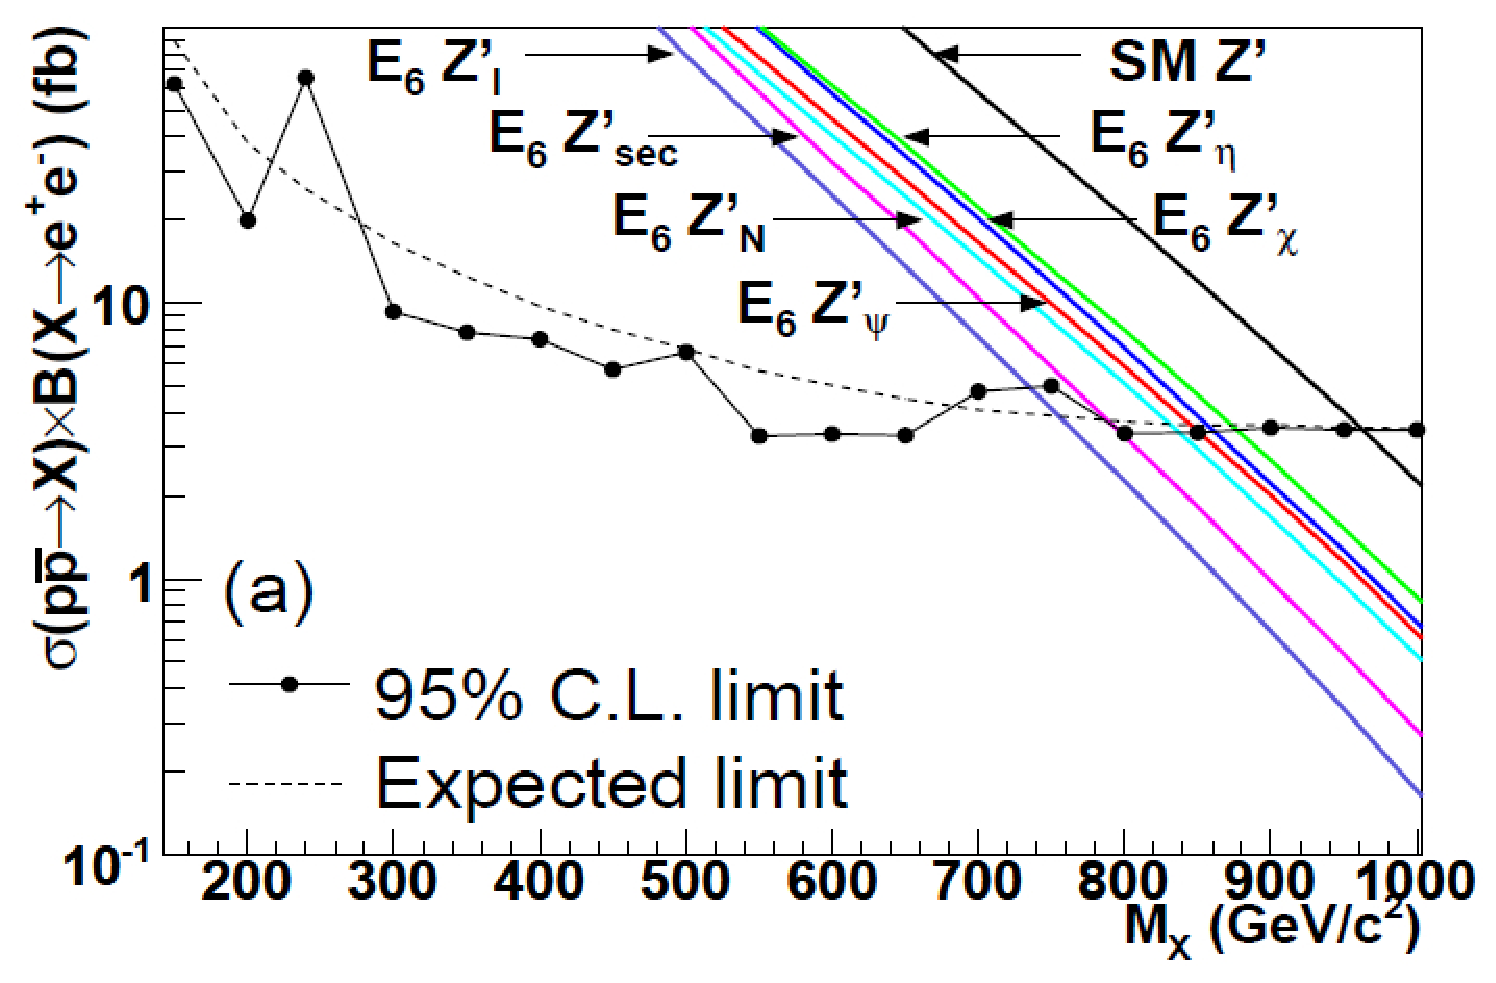
\includegraphics[width=0.47\textwidth]{figuras/Chapter1/CDFZprime2dielectronfigure.pdf}
      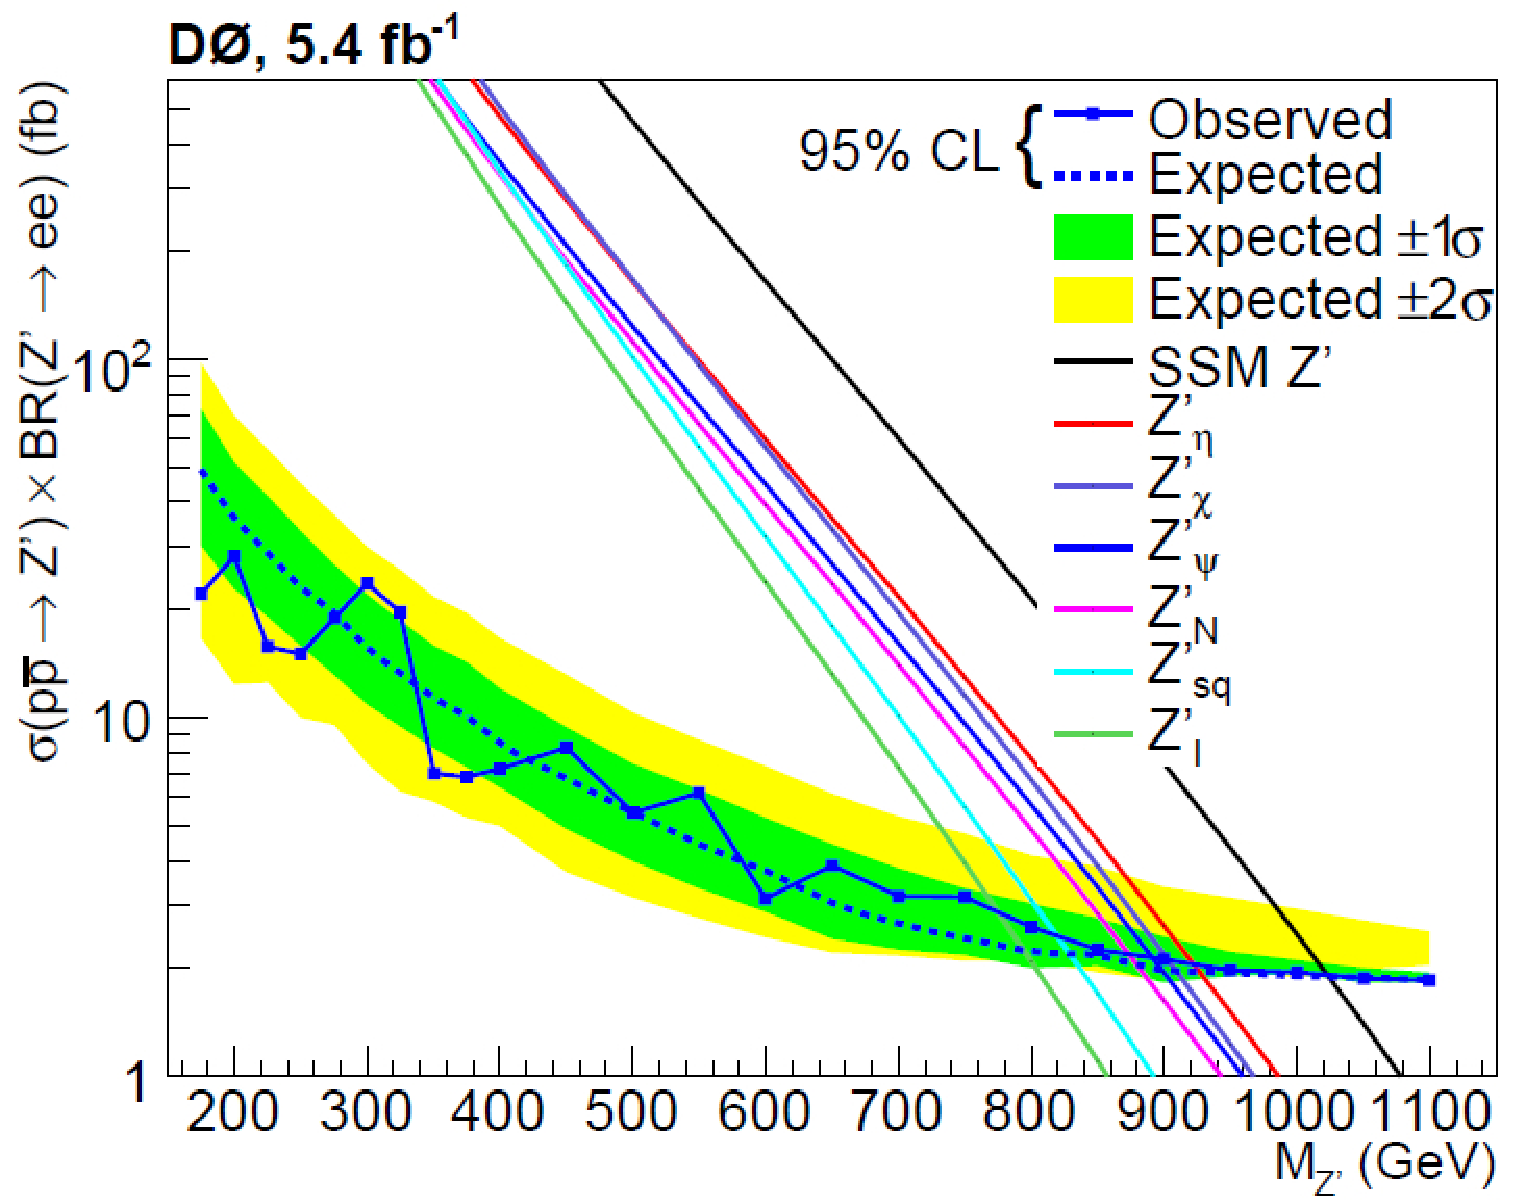
\includegraphics[width=0.45\textwidth]{figuras/Chapter1/D0Zprime2dielectronfigure}
      \caption{The figures show the 95$\%$ C.L. upper limits on
      $\sigma(p\bar{p}\rightarrow \text{Z}^{\prime})\times B(\text{Z}^{\prime}\rightarrow ee)$
      as a function of $M_{\text{Z}^{\prime}}$, compared to the theoretical predictions
      of the cross section for the \ZprimeSSM~and the bosons arising from E$_{6}$. (Left) Upper limits
      observed by CDF \cite{CDFZprimedielectronbib}. (Right) Upper limits observed by D0 \cite{D0Zprimetodielectronbib}.
      } \label{CDFD0dielectronresult}
    \end{center}
\end{figure}

\noindent The CMS and ATLAS experiments have performed searches for high-mass resonances in
the di-lepton channel using each data taking period \cite{CMSZprimetodileptonrun1run2, CMSZprimetodileptonrun1, CMSZprimetodileptonrun1sqrt7,
ATLASZprimetodileptonrun2, ATLASZprimetodilepton2015, ATLASZprimetodilepton2012, ATLASZprimetodileptonrun1}. The most recent
search performed by the CMS experiment combines the data collected during the years 2012 and 
2015 \cite{CMSZprimetodileptonrun1run2}. For the di-electron channel, the possible 
existence of a \Zprime~resonance is excluded up to 2.95 \TeV~for the \ZprimeSSM~and up to 
2.60 \TeV~for the \Zprimepsi. For the di-muon channel, the CMS Collaboration
 reports an absence of resonances in the di-electron mass spectrum below 3.22
\TeV~for \ZprimeSSM~and 2.67 \TeV~for \Zprimepsi. The combined analysis
provides an exclusion limit of 3.37 \TeV~and 2.82 \TeV~for \ZprimeSSM~and 
\Zprimepsi, respectively (see Figure \ref{CMSATLASdileptonresult}, left). On the other hand, 
the most recent search for \Zprime~bosons decaying into the di-lepton channel performed 
by the ATLAS experiment uses the data collected during 2015 and 2016 \cite{ATLASZprimetodileptonrun2}. The ATLAS 
Collaboration has excluded, with a 95$\%$ Confidence Level (CL), the mass of \ZprimeSSM~below 4.3 \TeV~in the
di-electron channel and 4.0 \TeV~in the di-muon channel, while the mass of \Zprimepsi~has been excluded for masses
below 3.9 \TeV~and 3.6 \TeV~in the di-electron channel and in the di-muon channel, respectively. The analysis with the 
combined channels results in an exclusion limit of 4.5 \TeV~for the \ZprimeSSM~boson and 3.8 \TeV~for 
\Zprimepsi~boson (see Figure \ref{CMSATLASdileptonresult}, right). The summary of the exclusion 
limits set on the \ZprimeSSM~and \Zprimepsi~for the di-lepton searches performed
by the CMS and ATLAS experiments are shown in Table \ref{tableCMSATLASdilepton}.\\


\begin{table}[ht]
\begin{center}
\begin{tabular}{|c|c|c|c|c|}   \hline   \hline
        
          & \multirow{2}{*}{\shortstack[c]{$\sqrt{s}$ [TeV]}} &  \multirow{2}{*}{\shortstack[c]{$\mathscr{L}$ [fb$^{-1}$] }} 
          & \multirow{2}{*}{\shortstack[c]{ Upper Limit \\ for \ZprimeSSM~[\TeV]}} &  \multirow{2}{*}{\shortstack[c]{Upper Limit \\ for \Zprimepsi~[\TeV]}} \\
%          &      &    $\mathscr{L}$ [fb$^{-1}$]    &   Upper Limit for \ZprimeSSM [TeV] & Upper Limit for \Zprimepsi [TeV] \\ \hline \hline
          &      &       &   &  \\ \hline \hline
  CMS     &      8 and 13      &  27 for $ee$ and 29 for $\mu \mu$ &               4.3                  &           3.9                    \\ \hline
  ATLAS   &         13         &             36                  &               4.5                  &           3.8                    \\ \hline \hline
\end{tabular}
\end{center}
\caption{Summary of the upper 95$\%$ CL limits set for \ZprimeSSM~and \Zprimepsi~masses in the di-lepton channel by the CMS and ATLAS experiments.}\label{tableCMSATLASdilepton}
\end{table}


\begin{figure}[ht]
\begin{minipage}[b]{0.4\linewidth} %Una minipágina que cubre la mitad de la página
\centering
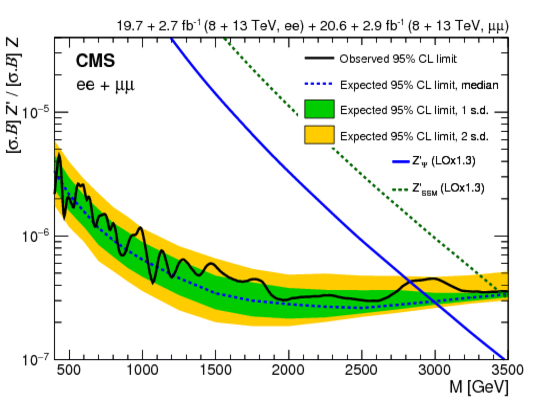
\includegraphics[width=7.5cm]{figuras/Chapter1/CMSZprime2dileptonRun2Run12}
\end{minipage}
\hspace{0.5cm} % Si queremos tener un poco de espacio entre las dos figuras
\begin{minipage}[b]{0.6\linewidth}
\centering
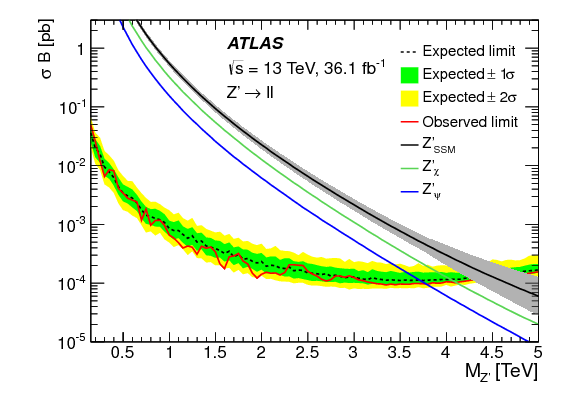
\includegraphics[width=7.5cm]{figuras/Chapter1/ATLASZprime2dilepton.png}
\end{minipage}
\caption{(Left) Upper 95$\%$ CL limits as a function of the resonance mass 
M on the ratio of the product of cross section and branching fraction into 
lepton pairs relative to that of Z bosons, for the combined 8 and 13 \TeV~data collected by CMS. Theoretical 
predictions for \ZprimeSSM~and \Zprimepsi~are shown for comparison \cite{CMSZprimetodileptonrun1run2}. (Right) Observed upper cross-section 
times branching ratio limits at 95$\%$ CL for \Zprime, E6-motivated \Zprimepsi~and \Zprimechi~bosons
using the combined di-lepton channel, for the combined 2015 and 2016 data collected by ATLAS. 
In addition, theoretical cross-sections are shown for the same models \cite{ATLASZprimetodileptonrun2}.} \label{CMSATLASdileptonresult}
\end{figure}

%\begin{center}
%\begin{figure}[ht]
%\centering
%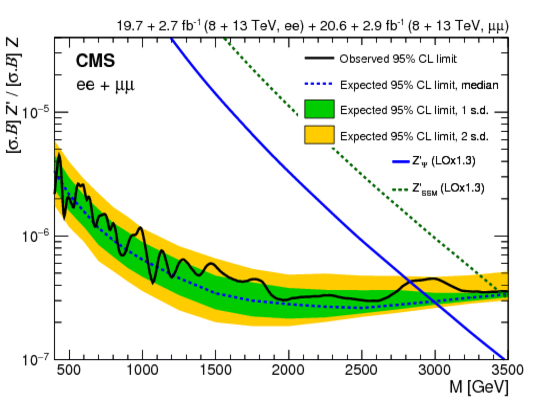
\includegraphics[scale=0.36]{figuras/Chapter1/CMSZprime2dileptonRun2Run12}
%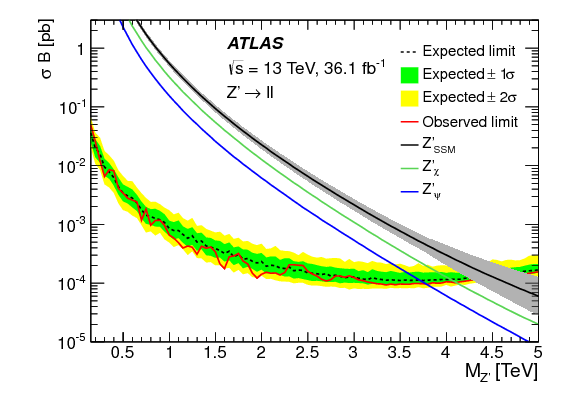
\includegraphics[scale=0.37]{figuras/Chapter1/ATLASZprime2dilepton.png}
%\caption{(Left) Upper 95$\%$ CL limits as a function of the resonance mass M on the ratio of 
%the product of cross section and branching fraction into lepton pairs relative to that of Z bosons,
%for the combined 8 and 13 \TeV~data collected by CMS. Theoretical 
%predictions for \ZprimeSSM~and \Zprimepsi~are shown for comparison \cite{CMSZprimetodileptonrun1run2}. (Right) Observed upper cross-section 
%times branching ratio limits at 95$\%$ CL for \Zprime, E6-motivated \Zprimepsi~and $Z_{\chi}$ bosons
%using the combined dilepton channel, for the combined 2015 and 2016 data collected by ATLAS. 
%In addition, theoretical cross-sections are shown for the same models \cite{ATLASZprimetodileptonrun2}.} \label{CMSATLASdileptonresult}
%\end{figure}
%\end{center}

\item \textbf{Di-tau searches (\Zprimetotautau~channel).}\\

\noindent The CMS and ATLAS Collaborations have provided the most stringent limits on 
the \Zprime~mass using the di-lepton channel. However, some models predict 
\Zprime~bosons which would couple preferentially to the third-generation of fermions, and hence, 
they would decay typically into tau pairs (see TAT models in section \ref{sec:Models}). In 
consequence, these models are the main motivation of searching for \Zprime~bosons decaying into taus. 
Additionally, if these hypothetical bosons were observed using another fermion channel, such as \Zprimetoll, 
the searches for \Zprimetotautau~would reveal the nature of its couplings (if it 
obeys or not the hypothesis of the universality of couplings). The benchmark models used 
for the search in this channel are \ZprimeSSM~and \ZprimeTAT. \\

\noindent The hypothetical \Zprimetotautau~events consist of 
two oppositely-charged high \pt~taus, produced back-to-back in the transversal 
direction. The searches for \Zprime~bosons in this channel involve different experimental 
signatures since, as will be explained further in section \ref{sec:Taus}, the tau can decay leptonically or 
hadronically, depending if its decay products are leptons ($\tau_{\ell}$) or 
hadrons ($\tau_{h}$). Then, this search usually is performed with the combination of four 
of the possible signatures: when both taus decay hadronically \Zprimetotauh; when one tau decays 
leptonically and the other one decays hadronically,
\Zprimetotaue~and \Zprimetotaumu; and when both taus decay leptonically \Zprimetoemu. They contribute 
approximately to a 94$\%$ of the \Zprime~decay branching fraction (this theses is focused on 
the \Zprimetotauh~channel). These searches is challenging from the experimental point 
of view since taus decay 66$\%$ of the times into hadrons; then, their signatures are 
similar than the ones produced by QCD jets. In consequence, the main background for theses 
channel comes from QCD processes, which are not well modeled by simulation, and data-driven 
techniques must be used to estimate their contribution. \\


%The signature of  consists on high \pt~tau pairs, which have 
%opposite charges and travel in opposite directions. 


\noindent Several searches for \Zprime~bosons decaying into  $\tau-$pairs have 
been performed by the CDF \cite{CDFZprimeditaubib} experiment at the Tevatron, and by the 
CMS \cite{CMSZprimetotautaurun1, CMSZprimetotautauemu, CMSZprimetotautau2015} and 
ATLAS \cite{ATLASZprimetotautau2016, ATLASZprimetotautau2015, ATLASZprimetotautaurun1, ATLASZprimetotautau2011} experiments 
at the LHC. The CDF Collaboration excluded the \ZprimeSSM~boson in the di-tau channel
for masses below 399 \GeV, using 195 fb$^{-1}$ of collected data from \cite{CDFZprimeditaubib}. \\

\noindent The tightest constraints on the \Zprime~mass using the di-tau channel have 
been set by the CMS and ATLAS Collaborations. For this channel, CMS has performed the search combining the four
 tau signatures mentioned above (\tauh \tauh,~\taue \tauh,~\taumu \tauh~and \taue \taumu)
with the data collected during 2011, which corresponds to pp collisions at \sqrts7 \TeV~with 
an integrated luminosity of 4.9 fb$^{-1}$. Upper limits were reported on the production of \Zprime, excluding 
its existence with 95$\%$ CL below 1.4 \TeV~for \ZprimeSSM~and 1.1 \TeV~for \Zprimepsi~\cite{CMSZprimetotautaurun1}. Additionally, 
the CMS Collaboration has carried out the search for \Zprime~bosons in the $\tau_{e}\tau_{\mu}$ channel; this search 
was performed with the data collected during 2012, which corresponds to 19.7 fb$^{-1}$ of pp collisions at \sqrts~8 \TeV
As a result, \ZprimeSSM~and \Zprimepsi~were excluded for masses below 1.3 \TeV~and 0.81 \TeV 
respectively \cite{CMSZprimetotautauemu}. The \Zprimetotautau~search was also performed with the data collected
by CMS during 2015, combining the four di-tau signatures mentioned above. This search, which uses pp collisions 
at \sqrts13 \TeV~with an integrated luminosity of 2.2 fb$^{-1}$, set upper 95$\%$ CL limits for 
\ZprimeSSM~masses below 2.1 \TeV~and \ZprimeTAT~masses below
1.7 \TeV~(see Figure \ref{CMSditauresult}, right) \cite{CMSZprimetotautau2015}. The exclusion limits 
set by the \tauh \tauh~channel constrain the existence of the \ZprimeSSM~for masses up to 
1.92 \TeV~and the \ZprimeTAT~for masses up to 1.51 \TeV~(see Figure \ref{CMSditauresult}, left). The search 
performed in the \tauh\tauh~channel is specially important since it will serve as a reference for the 
analysis performed in this thesis. \\ %Since some of the cuts have been changed and there is more statistics

\begin{center}
\begin{figure}[ht]
\centering
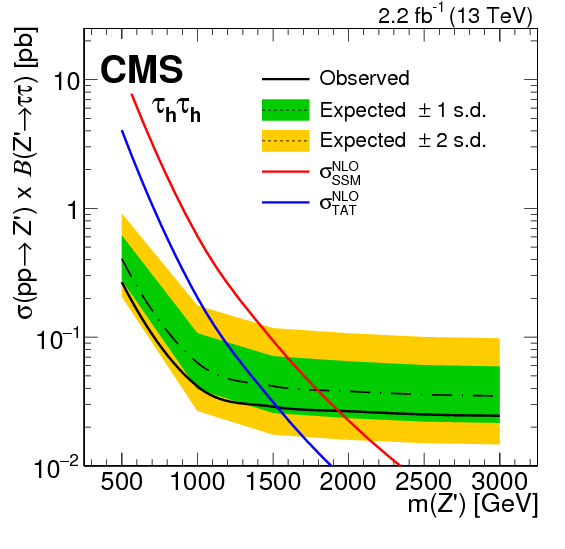
\includegraphics[scale=0.36]{figuras/Chapter1/CMSZprime2ditauhRun2.png}
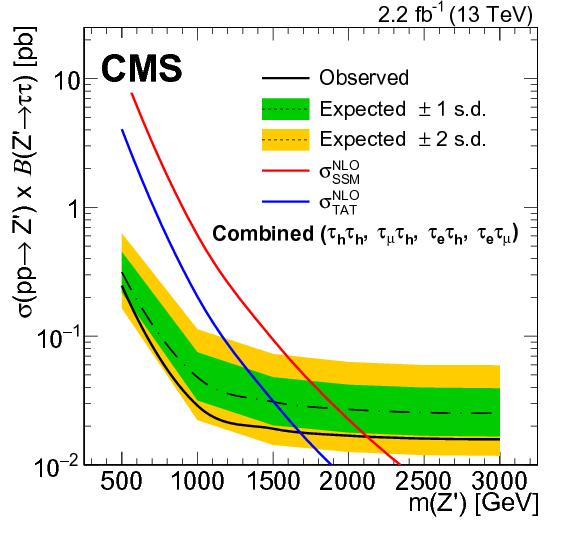
\includegraphics[scale=0.36]{figuras/Chapter1/CMSZprimeditauRun2.png}
\caption{Upper limit at the 95$\%$ CL on the product of the cross section and
branching fraction into $\tau$ pairs as a function of the \Zprime~mass. The bands represent the
one and two standard deviations. The figure shows the results by the CMS Collaboration
for the \tauh \tauh~channel  (left) and the combination of four 
di-tau channels: \tauh \tauh,~\taue \tauh,~\taumu \tauh~and \taue \taumu (right) \cite{CMSZprimetotautau2015}.
} \label{CMSditauresult}
\end{figure}
\end{center}


\noindent The ATLAS Collaboration has reported the tightest exclusion limits on the 
\Zprime~mass using the di-tau channel since the search was performed with the data 
collected during 2015 and 2016, using pp collisions at \sqrts~13 \TeV~with an integrated 
luminosity of 36.1 fb$^{-1}$; ATLAS has excluded the \ZprimeSSM~for masses below 2.42 \TeV~
with 95 $\%$ CL (See Figure \ref{ATLASditauresult}, right)\cite{ATLASZprimetotautau2016}. The summary of the exclusion 
limits set on the \ZprimeSSM~mass in the di-tau searches, performed by CMS and ATLAS experiments, 
are shown in Table \ref{tableCMSATLASditau}.\\

\begin{table}[ht]
\begin{center}
\begin{tabular}{|c|c|c|c|c|c|}   \hline   \hline
        
\multirow{2}{*}{\shortstack[c]{}}      &    \multirow{2}{*}{\shortstack[c]{Data}}      & \multirow{2}{*}{\shortstack[c]{\sqrts [\TeV]}} &  \multirow{2}{*}{\shortstack[c]{$\mathscr{L}$ [fb$^{-1}$] }} 
          & \multirow{2}{*}{\shortstack[c]{ di-tau \\ channel}}  & \multirow{2}{*}{\shortstack[c]{ Upper Limit \\ for \ZprimeSSM~[\TeV]}}  \\
                                     &          &      &        &                                                        &  \\ \hline \hline
\multirow{3}{*}{\shortstack[c]{CMS}} &   2011   &   7  &   4.9  &  \tauh \tauh, \taue \tauh, \taumu \tauh, \taue \taumu  &  1.4  \\ \cline{2-6}
                                     &   2012   &   8  &  19.7  &   \taue \taumu                                         &  1.3  \\ \cline{2-6}
                                     &   2015   &  13  &   2.2  &  \tauh \tauh, \taue \tauh, \taumu \tauh, \taue \taumu  &  2.1  \\ \hline \hline 
                      ATLAS &   2015 and 2016   &  13  &   36.1  & \tauh \tauh, \taue \tauh, \taumu \tauh                &  2.4  \\ \hline \hline 
\end{tabular}
\end{center}
\caption{Summary of the upper 95$\%$ CL limits set for \ZprimeSSM~and \Zprimepsi~masses in the di tau channels by the CMS and ATLAS experiments.}\label{tableCMSATLASditau}
\end{table}


\begin{center}
\begin{figure}[ht]
\centering
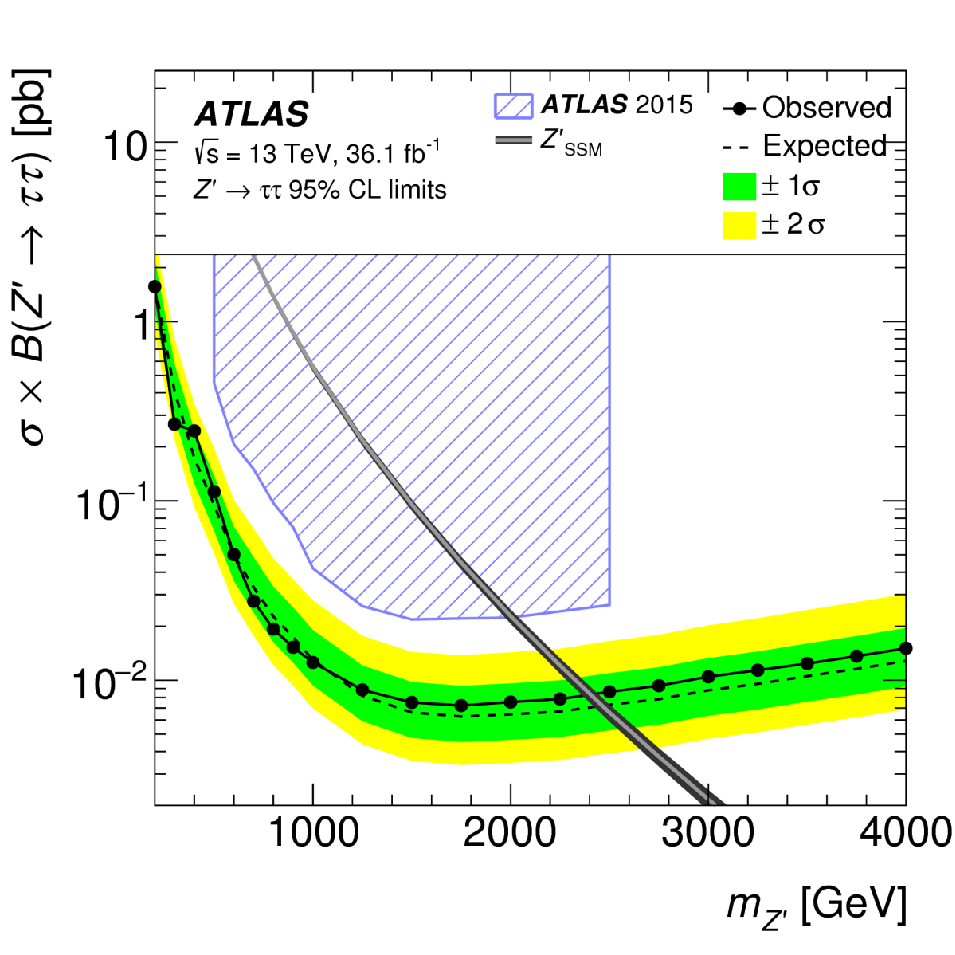
\includegraphics[clip,width=0.47\textwidth]{figuras/Chapter1/ATLASZprime2ditaufigure.pdf}
\caption{Upper limit at the 95$\%$ CL on the product of the cross section and
branching fraction into $\tau$ pairs as a function of the \Zprime~mass. The bands represent the
one and two standard deviations. The figure shows the results by the ATLAS Collaboration \cite{ATLASZprimetotautau2016}.
} \label{ATLASditauresult}
\end{figure}
\end{center}


\item \textbf{Di-jet (\Zprime~$\rightarrow q\bar{q}$) searches.}\\

\noindent Since \Zprime~bosons might decay into quark-antiquark pairs, the CMS and
ATLAS Collaborations have reported several searches that involve 
a jet-pair such as:  $t\bar{t}$ \cite{CMSZprimetotoptoprun1}, $b\bar{b}$ \cite{CMSZprimetodibjetsrun1,ATLASZprimetobjet2015}
and $jj$ \cite{CMSZprimedijetrun2,ATLASZprimetojet2015}. The copious 
contribution of background from QCD processes degrades the mass-resolution, making 
these channels less sensitive than the di-lepton ones. In these searches the exclusion
limits go from from 1 \TeV~to 2.7 \TeV depending on the 
model (see the references quoted before for more details.)
\end{itemize}

\textbf{Summary}. \\

\noindent In summary, the searches for \Zprime~bosons have not resulted in any confirmed observation,
nor in any significant deviations from SM predictions, that would suggest their existence. Only
lower exclusion limits on their masses have been set. The tightest limits on the \Zprime~mass
have been set by the CMS and ATLAS Collaborations in the di-lepton channel, where the 
\ZprimeSSM~and \Zprimepsi~bosons have been excluded for masses below 3.37 \TeV~and 2.82 \TeV respectively.
Nevertheless, several BSM scenarios predict \Zprime~bosons that may have weak couplings with
electrons and muons, and might decay preferably into $\tau-$pairs. The CMS and ATLAS experiments
performed searches on \Zprime~decaying into $\tau\tau$ using samples from Run II, and 
have excluded the \ZprimeSSM~mass below 2.1 \TeV~(CMS) and 2.4 \TeV~(ATLAS). The purpose of this thesis
is to search for \Zprime~bosons decaying into $\tau_{h}\tau_{h}$ using the data recorded by CMS during 2016.

\section{The Physics of the tau-lepton}
\label{sec:Taus}

\noindent Since the final state of the channel analyzed in this work involves 
taus, some of the properties of this particle are presented 
in this section. The tau-lepton belongs to the third generation of fermions and is the 
heaviest lepton, with a mass of 1.777 \GeV. It has a lifetime of 2.9 $\times$ 10$^{-13}$ s, and its 
decay length, $c\tau$, is 87 $\mu$m. It is the only lepton with enough mass 
to decay into leptons but also into hadrons. At the fundamental 
level, a $\tau$ decays into a neutrino by the emission of an off-shell 
W boson ($\tau \rightarrow \nu_{\tau} \text{W}^*$). The W$^*$ decays $33\%$ of the times
leptonically, W$^* \rightarrow \nu_{\ell} \ell$ ($\ell = e,\mu$); and it decays 
hadronically the remaining $67\%$ of the times, W$^* \rightarrow q \bar{q}$. 
In the hadronic case the $q\bar{q}$ pair will form hadrons (mostly pions). Figure \ref{taudecays} shows the 
the Feynman diagrams of the tau decays and the branching fraction of the tau decay modes is 
listed  in Table \ref{tab:taudecaymodes}. \\

% the Feynman diagrams of the tau decays and the branching fraction of each tau decay mode is 
% listed in Table \ref{tab:taumods}. \\

%summary, the decay modes of the $\tau$ can be classified as:

%a tau neutrino 
%by the emission of an off-shell W boson; therefore, taus can decay 
%leptonically, \tauell~($\ell$ $=$ $e, \mu$), or hadronically, \tauh, depending on 
%the W boson decay products since it decays around $33\%$ of the times into the lighter leptons and a neutrino, and 
%the remaining  $66\%$ into the lighter quarks. Figure \ref{taudecays} shows the 
%the Feynman diagrams of the tau decays. The branching fraction of each 
%tau decay is listed in Table \ref{tab:taumods}. \\

%The tau can decay into leptons through: 
%$\tau \rightarrow \nu_{\tau}\ell \bar{\nu}_{\ell}$

\begin{center}
\begin{figure}[ht]
\centering
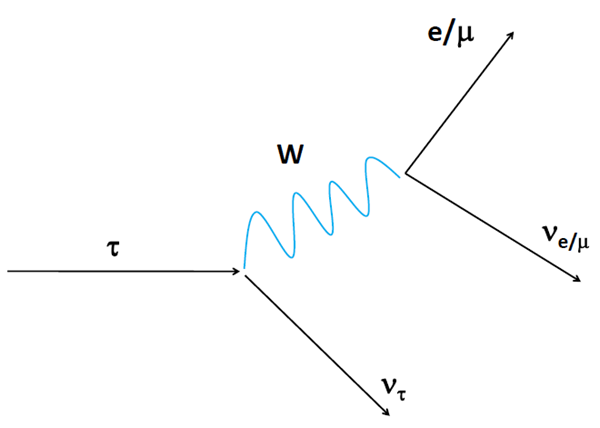
\includegraphics[scale=0.6]{figuras/Chapter1/leptondecay.png}
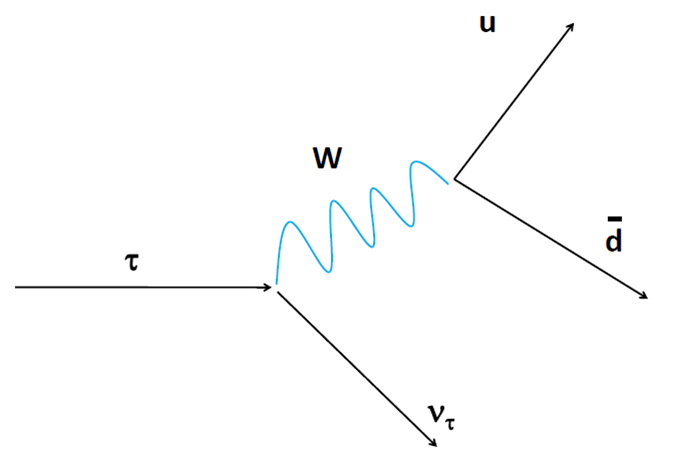
\includegraphics[scale=0.5]{figuras/Chapter1/hadrondecay.png}
\caption{Feynman diagrams of the tau decays: on the left, the tau leptonic decay (\tauell) and on the right,
the hadronic decay (\tauh).
} 
\label{taudecays}
\end{figure}
\end{center}

%\noindent The hadronic decay of taus involves a relative small number of hadrons 
%compared with the ones produced by QCD-jets.

%a well known number of 
%charged hadrons since tau can decay into meson resonances, which contrasts 
%with the copious amount of charged particles coming from the 
%hadronizacion process of a single quark. 

%  \begin{table}[ht]
%   \centering{
%  \begin{tabular}{|l|c|}
%    \hline
%    Tau decay mode                                          &  Braching Fraction [$\%$]    \\ \hline\hline
%    $e^{-}\bar{\nu}_{e}\nu_{\tau}$                          & 17.83 $\pm$ 0.04             \\ \hline
%    $\mu^{-}\bar{\nu}_{\mu}\nu_{\tau}$                      & 17.41 $\pm$ 0.04             \\ \hline
%    hadronic decays                                         & 64.79 $\pm$ 0.06            \\ \hline
%    \hline
%  \end{tabular}
%  \caption{Branching fraction of $\tau^{-}$ modes\cite{PDG}.}
%  }
%  \label{tab:taumodes}
%  \end{table}
%  
  \begin{table}[ht]
  \begin{center}
  \begin{tabular}{|l|c|}
    \hline
    Tau decay mode                                          &  Branching Fraction [$\%$]    \\ \hline\hline
    $e^{-}\bar{\nu}_{e}\nu_{\tau}$                          & 17.83 $\pm$ 0.04             \\ \hline
    $\mu^{-}\bar{\nu}_{\mu}\nu_{\tau}$                      & 17.41 $\pm$ 0.04             \\ \hline
    hadronic decays                                         & 64.79 $\pm$ 0.06            \\ \hline
    \hline
  \end{tabular}
  \caption{Branching fraction of $\tau^{-}$ modes \cite{bib:PDG}.} 
  \label{tab:taudecaymodes}  
  \end{center}

  
%    \caption{Branching fraction of $\tau^{-}$ modes \cite{particledatagroup}.} \label{tab:taudecaymodes}

%   \caption{Branching.}

\end{table}

% \begin{table}[ht]
% \begin{center}
% \begin{tabular}{|l|c|c|c|}
%   \hline
%   Final State                                             &  Braching Fraction [$\%$] &  Resonance & Mass [\GeV]   \\ \hline\hline
%   $e^{-}\bar{\nu}_{e}\nu_{\tau}$                          & 17.83 $\pm$ 0.04          &            &   \\ \hline
%   $\mu^{-}\bar{\nu}_{\mu}\nu_{\tau}$                      & 17.41 $\pm$ 0.04          &            &   \\ \hline
%   $\pi^{-}\nu_{\tau}$                                     & 10.83 $\pm$ 0.06          &            &   \\ \hline
%   $\pi^{-}\pi^{0}\nu_{\tau}$                              & 25.52 $\pm$ 0.09          & $\rho$     & 770 \\ \hline
%   $\pi^{-}\pi^{0}\pi^{0}\nu_{\tau}$                       &  9.30 $\pm$ 0.11          & $a_{1}$    & 1200  \\ \hline
%   $\pi^{-}\pi^{0}\pi^{0}\pi^{0}\nu_{\tau}$                &  1.05 $\pm$ 0.07          &            &   \\ \hline
%   $\pi^{-}\pi^{-}\pi^{+}\nu_{\tau}$                       &  8.99 $\pm$ 0.06          & $a_{1}$    & 1200  \\ \hline
%   $\pi^{-}\pi^{-}\pi^{+}\pi^{0}\nu_{\tau}$                &  2.70 $\pm$ 0.08          & $a_{1}$    & 1200  \\ \hline
%   \hline
% \end{tabular}
% \end{center}
% \caption{Branching fraction of $\tau^{-}$ modes\cite{PDG}.}\label{tab:taumodes}
% \end{table}


\noindent The tau identification is challenging from the experimental point of view
for several reasons. As was mentioned above, the final states of the tau decays involve
one or two neutrinos; however, it is not possible to observe neutrinos without 
an enormous amount of material and therefore, they can not be detected in experiments 
like CMS. As consequence, a fraction of the tau 4-momentum goes undetected, not allowing 
the full reconstruction of its kinematical parameters. Additionally, due to the relative 
small decay length, it is not possible to distinguish the tau decay vertex from 
the primary vertex of the collision. Therefore, in the leptonic case, the presence of 
neutrinos and the absence of a secondary vertex makes it impossible 
to distinguish a charged lepton coming from a tau decay than one coming 
from other processes. In consequence, taus can only be identified directly 
from their hadronic decays. \\

\noindent The hadronic identification of taus is also challenging since 
the experimental signature is similar to the one of hadronic-\textit{jets}.
An hadronic-jet, or QCD-jet, comes from the strong interactions between 
quarks and leptons, resulting in an abundant amount of charged and neutral 
pions emitted within a cone. Since the \tauh~decay produces a neutrino 
plus pions (charged an neutral ones), they can be misidentified as a QCD-jets.
Besides, these jets are produced copiously in pp collisions and their yield is 
eight orders of magnitude higher than the one of \tauh, constituting a large
source of background for the tau identification. Nevertheless, there are some 
differences between a \tauh~and a QCD jet, that allow for a good level
of discrimination: for instance, a QCD jet has a wider energy profile than a \tauh;
the hadronic tau decay also have a narrower cone and fewer charged particles 
than the QCD jets. These differences can be exploited to implement 
algorithms in order to distinguish between them. \\

\noindent Since the purpose of this work is to search for \Zprime~bosons
in the di-hadronic tau decay channel, the tau identification in 
the CMS experiment is crucial. Chapter \ref{chap:CMSExp}
describes the CMS experiment, with an special focus on the 
experimental signatures of the tau decay products, and Chapter
\ref{chap:ParticleID} shows the algorithms used for CMS in order identify 
the particles that emerge from a collision, making emphasis 
in the tau identification algorithm, which is described in section \ref{sec:RecoTau}. \\


%Even more, a vertex is reconstructed using at 
%least two charged-particle tracks; therefore, in the 
%leptonic case, that only includes one charged lepton ($\ell = e, \mu$), 
% both, the $e$ and the $\mu$ cannot be distinguished from those coming from the collision.

%in the leptonic decay case, the $e$ and the $\mu$ cannot be distinguished 
%from those coming from the collision.

%In consequence, it is not possible to identify a $\tau_{\ell}$ individually; it can be 
%done only in the context of the complete kinematic information of the final state of the event. \\




%Since the tau can decay
%leptonically into a lighter charged lepton and two neutrinos ($\tau_{e}$, $\tau_{\mu}$), or
%hadronically into a neutrino plus pions ($\tau_{h}$), a search of a Z$'$ boson
%includes the Z$'\rightarrow\tau_{h}\tau_{h}$, Z$'\rightarrow\tau_{h}\tau_{\mu}$,
% Z$'\rightarrow\tau_{h}\tau_{e}$ and Z$'\rightarrow\tau_{e}\tau_{\mu}$ decay modes. The
% channels Z$'\rightarrow\tau_{\mu}\tau_{\mu}$ and Z$'\rightarrow\tau_{e}\tau_{e}$ are
 

